\title{Independent Research: History of The Proton Radius}
\author{
        Ethan Rooney \\
                Department of Physics\\
        George Washington Univerisity\\
        Washington D.C., 20052
}
\date{\today}

\documentclass[12pt]{article}
\usepackage{array}
\newcolumntype{L}{>{\centering\arraybackslash}m{1.8cm}}
\usepackage{amsmath}
\usepackage{graphicx}
\usepackage{epigraph}
\graphicspath{ {.images/} }

\begin{document}
\maketitle

%\begin{abstract}
%\end{abstract}

\section{Introduction}
Historical context, Contemporary Experiments, Future of MUSE.

\section{Rutherford, Gold Foil, Impossible Results}

Dr. Hans Geiger and an undergraduate assistant, Ernest Marsden, constructed an experiment to assist Ernest Rutherford in probing the structure of the nucleus.
The experimental apparatus was ingenious and deceptively simple.

\begin{figure}[h]
    \centering
    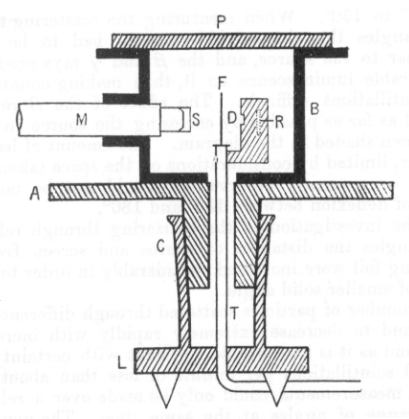
\includegraphics[width=7cm]{gold_foil_device}
    \caption{Geiger-Marsden $\alpha$ scattering device\cite{Geiger1913}}
    \label{fig:device}
\end{figure}

In Figure \ref{fig:device} we see a cross section of the device used to gather the distribution of $\alpha$ particles scattered from a thin metal foil.
The device consisted of an evacuated box B, inside of which there was a Radium $\alpha$ source R, and a gold foil F.
Between the $\alpha$ source and foil was a collimating diaphragm, that only allowed a small "pencil of $\alpha$ particles" to be incident on the foil.
The experimenter could then look at a screen coated in a substance that would let out a pulse of light, in a processes known as scintillation, when struck by a charged particle. This scintillation screen S was attached to the end of microscope M.
The microscope and scintillation screen could be rotated around the foil and $\alpha$ source, allowing for the experimenter to collect events at an arbitrary scattering angle. 
Whenever a scattered particle deflected into the observed angle,the scintillator coating would light up, and each of these scintillations would then be tallied by hand.
For several of the experiments, Geiger and Marsden collected data from 5 degrees to 150 degrees off of the beam line. This allowed them to measure the number of scintillations as a function of order the scattering angle.This function of the number of scatterings by scattering angle is called the differential cross section.
We can see the some of the data they collected for an experiment run with both a gold foil and a silver foil in Table \ref{table:gvs}.


\begin{table}[h]
    \begin{tabular}{|L|L|L|L|L|L|}
        \hline
          &  & \multicolumn{2}{c|}{Silver Foil} &\multicolumn{2}{c|}{Gold Foil} \\ \cline{3-6}
        Angle of deflection $\phi$ & $\frac{1}{\sin^4{\phi/2}}$ & Number of Scintillations, $N$ & $\frac{N}{\sin^4{\phi/2}}$ & Number of Scintillations, $N$ & $\frac{N}{\sin^4{\phi/2}}$\\
        \hline
        150&1.15&22.2&19.3&33.1&28.8\\
        135&1.38&27.4&19.8&43.0&31.2\\
        120&1.79&33.0&18.4&51.9&29.0\\
        105&2.53&47.3&18.7&69.5&27.5\\
        75&7.25&136&18.8&211&29.1\\
        60&16.0&320&20.0&477&29.8\\
        45&46.6&989&21.2&1435&30.8\\
        37.5&93.7&1760&18.8&3300&35.3\\
        30&223&5260&23.6&7800&35.0\\
        22.5&690&20300&29.4&27300&39.6\\
        15&3445&105400&30.6&13200&38.4\\
        \hline
    \end{tabular}
    \caption{Original Data as reported by Geiger and Rutherford \cite{Geiger1913}}
    \label{table:gvs}
\end{table}

In Earlier work Geiger, Marsden and Rutherford had shown that most $\alpha$ particles would undergo a small deflection when passing through a metal foil\cite{Geiger1908}. In this new experiment the team was measuring for was large angle deflections, especially those particles scatter greater than $90^\circ$.
These large deflections, known as backscatter, are significantly less likely to occur than the those at lesser angles.
About $1/8000$ events, undergoes a deflection of greater than $90^\circ$.
In 1908, a plum-pudding model of the atom was one of the leading explanations. 
This plum-pudding model had a diffuse cloud of positive charge, spread over the whole range of the influence of the atom ~$10^{-10}$ meters, with negative charges embedded inside.
This model, was frequently pictured as a sphere of constant positive charge, with small corpuscles of negative charge embedded inside. Like dried fruit in a dessert, hence a "plum-pudding".

This plum-pudding model had a problem.
In order for a charged particle to undergo a backscatter, the particle has to loose all of its forward momentum, slow to a stop in the direction of the beam and then turn back towards the source.
The kinetic energy carried by the $\alpha$ particle emitted by a decay of radium $4.87$ MeV.
This means that in order to stop the $\alpha$ particle, the electrostatic potential energy between the nucleus and $\alpha$ particle must be the same.
If the positive charge of the atom is distributed over the whole region of the atom, then the Electric field will be: 

\begin{equation}\label{eq:efield-diffuse}
    E = \frac{kQr}{R^3}\hat{r}
\end{equation}

Where k is the coulomb constant, Q is the charge of the atom, r is the distance from the center of the atom, and R is the radius of the atom. Using Equation \ref{eq:efield-diffuse} we can find the electrical potential and thus the potential energy of an $\alpha$ particle traveling inside the atom.

\begin{equation}
    \Delta{V} = V(R)-V(r) = -\int_r^RE\cdot{ds} = -\int_r^RE dr = \frac{-kQ}{R^3}\int_r^Rr dr
\end{equation}

\begin{equation}\label{eq:potential-diffuse}
    V(r) = \frac{kQ}{2R}(3-\frac{r^2}{R^2})
\end{equation}

Since the potential of a charged particle is given by $V\cdot{q}$ we can find the potential energy of a particle traversing the plum-pudding nucleus, as seen in Figure \ref{fig:plumenergy}

\begin{figure}
    \centering
    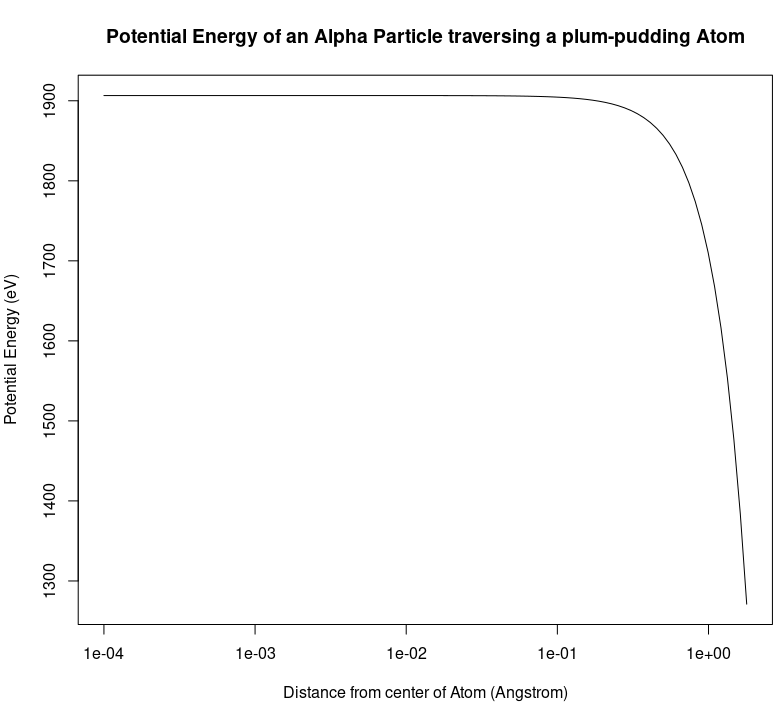
\includegraphics[width=10cm]{plumenergy}
    \caption{The Plum-Pudding model of an atom cannot generate the forces required to turn an $\alpha$ particle through a large angle}
    \label{fig:plumenergy}
\end{figure}


According to the leading physics of the time, backscatter of $\alpha$ particles from a thin gold foil was something that wasn't supposed to be possible.
The best understanding of the natural world said: the energy carried by alpha particles should allow them to punch right through the atoms of gold with only a tiny deflection.
Most of the time, that is exactly what happened.
$\alpha$ particles would pass through the foil with just the smallest of deflections ~$0.87^\circ$, but one out of every 20 thousand $\alpha$ particles would undergo a backscatter in a gold\cite{Rutherford1911}.
In the plum-pudding model, the electric field is not sufficient to backscatter the charged particles.

Rutherford, continued exploring this with another newly discovered particle, the $\beta$ particle.
From other experiments, he knew that the $\beta$ the opposite charge of the $\alpha$, but when fired into a gold foil, they behaved similarly.
Most $\beta$ particles passed through the foil, but some would experience a large deflection.


In order to solve this discrepancy Rutherford proposed a different model for the charge distribution inside the atom. 
The model he suggested is the model we are broadly familiar with today. A small dense object with a central positive charge, and orbiting electrons on the outside.
He also knew that, because of the charges involved, the electric field would only play a significant role if the $\beta$ particles penetrated inside of the electron layer. 
This result can be shown from Gauss's law in Equation \ref{eq:gauss}.

\begin{equation}\label{eq:gauss}
    \Phi_E = \frac{Q}{\varepsilon_0}
\end{equation}

In \ref{eq:gauss} $\Phi_E$ is the electric flux through a closed surface, $Q$ is the total charge, and $\varepsilon_0$ is the electric constant. Since the net charge of an atom is neutral, the $\Psi_E$ must be zero until you get inside of the orbitals of the atom.

Given this information we can see that the electric field and Electric potential must be as we see in Equations \ref{eq:potential} and \ref{eq:electricfield}

\begin{equation}\label{eq:potential}
V = Ne(\frac{1}{r} - \frac{3}{2R} + \frac{r^2}{2R^3})
\end{equation}

\begin{equation}\label{eq:electricfield}
E = -\frac{dV}{dr} = Ne(\frac{1}{r^2} - \frac{r}{R^3})
\end{equation}

Where V is the electric potential, E is the electric field, r is the distance from the center of the atom, R is the Radius of the electron orbits, k is the Coulomb constant, N is the Atomic Number, e is the elemental charge.

In the equation for the electric field above, the positive contribution is from the central charge, and the negative term is from the electrons surrounding it.
With this new model the field attains a strength high enough to turn some incoming particles around, while allowing for most particles coming in to undergo a relatively small deflection.

Let's take a look at what would happen to an $\alpha$ on a collision course. $\alpha$ particle fired directly at the central charge, with some velocity $v$, would carry the energy in Equation \ref{eq:KE}.

\begin{equation}\label{eq:KE}
    KE = \frac{1}{2}mv^2
\end{equation}

From a conservation of energy standpoint, the particle would have to come to a complete stop when the potential energy of system was equal to the initial kinetic energy. Given that the potential energy of a charged particle in a electric potential can be found with Equation \ref{eq:electricPE}.

\begin{equation}\label{eq:electricPE}
    PE = Vq = qNe(\frac{1}{r^2} - \frac{r}{R^3})
\end{equation}

Substituting Equation \ref{eq:KE} into Equation \ref{eq:electricPE} we get Equation \ref{eq:KEPE} below.

\begin{equation}\label{eq:KEPE}
    \frac{1}{2}mv^2 =  qNe(\frac{1}{r} - \frac{3}{2R} + \frac{r^2}{2R^3})
\end{equation}

Assuming r is very small compared to R when the particle stops, Equation\ref{eq:KEPE} can be simplified to Equation \ref{eq:KEPEsimple}

\begin{equation}\label{eq:KEPEsimple}
    \frac{1}{2}mv^2 = qNe(\frac{1}{r} - \frac{3}{2R})
\end{equation}

Thus we find the particle will come to rest when $r=[\frac{2qNe}{mv^2} + \frac{3}{2R}]^{-1}$.

This stopping distance, $b$, is important for the further derivation of the scattering angle expected from a point nucleus.



\begin{figure}
    \centering
    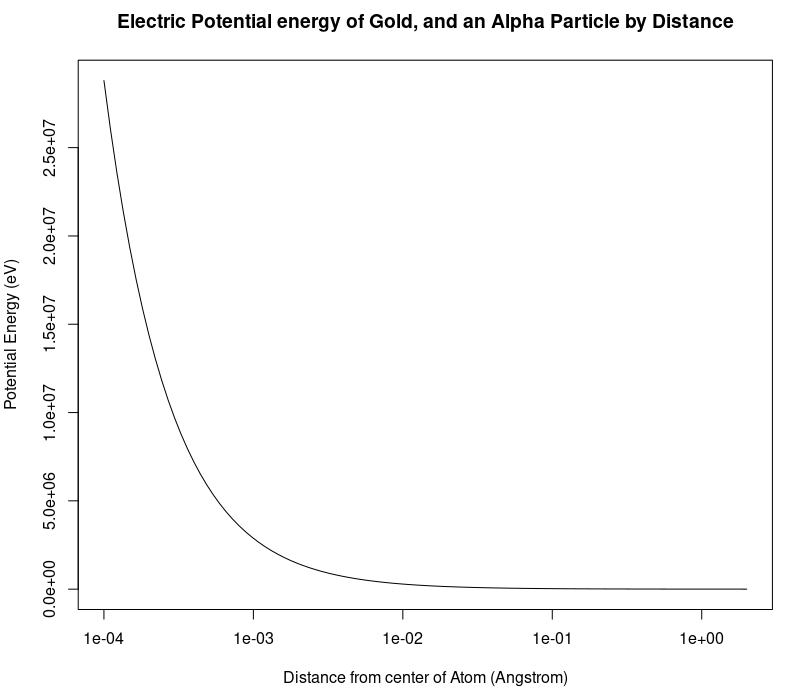
\includegraphics[width = 10cm]{ruthenergy}
    \caption{Potential Energy of a $\alpha$ particle as a function of the distance from the nucleus.}
    \label{fig:ruthenergy}
\end{figure}

As we can see in Figure \ref{fig:ruthenergy} the energy of a charged particle increases rapidly if the nucleus is sufficiently dense. This high central density makes it possible for large deflections to occur.

While $\alpha$ particles are useful in probing the structure of large atoms, they have an atomic mass of approximately $4$ amu.
This means that for probing the structure of small atoms, we can no longer make the assumption that no momentum is transferred into the target nucleus.
Additionally, when an $\alpha$ particle gets close to the target nucleus, the short range nuclear forces are no longer negligible.
Fortunately, another particle exists that has neither of these draw backs.
Electrons, and leptons broadly, are light particles that cannot interact with the nuclear forces, and therefore are able to be used in place of $\alpha$ particles.
Electrons, also called $\beta$ particles, have a rest mass of of $5.45*10^-4$ amu.

\section{Proton Radius, N.F. Mott, Relativity, and Dirac}

In 1920 Rutherford made another discovery fundamental to nuclear physics. He showed that when nitrogen gas was bombarded with $\alpha$ particles helium gas was generated. From this he was able to conclude that the positive charges in every atom were the same as that present in hydrogen gas\cite{Rutherford1920}. It was at this point that physicists turned their attention to measuring this basic building block.

If the particle at the center of a hydrogen atom was a point particle, we would expect the follow Rutherford's formula for differential cross-section Equation \ref{eq:rutherforddifcross}, at least for non-relativistic particles \cite{Hofstadter1956}

Because Rutherford's differential cross section equation \ref{eq:rutherforddifcross} breaks down at higher energies, it couldn't be used to distinguish from a highly compact object or one that was truly a point particle. For that we can turn to the theoretical work of N. F. Mott.

Mott expanded upon the work of Rutherford and extended Equation \ref{eq:rutherforddifcross} into a relativistic regime\cite{Hofstadter1956}.

\begin{equation}\label{eq:rutherforddifcross}
    \sigma(\theta) = \frac{q^2Q^2e^4}{16E^2\sin^4(\frac{\theta}{2})}
\end{equation}

\begin{equation}\label{eq:mottscatter}
    \sigma_M(\theta) = (\frac{Ze^2}{2mc^2})^2(\frac{1-\beta^2}{\beta^4})\frac{1}{\sin^4{\frac{\theta}{2}}}(1-\beta^2\sin^2\frac{\theta}{2})
\end{equation}

With this new relativistic model Mott could now make very precise predictions on the behavior higher energy electrons scattered from a point particle, and experimentalists like Hofstadter had new experiments to test those predictions. 

\begin{figure}
    \centering
    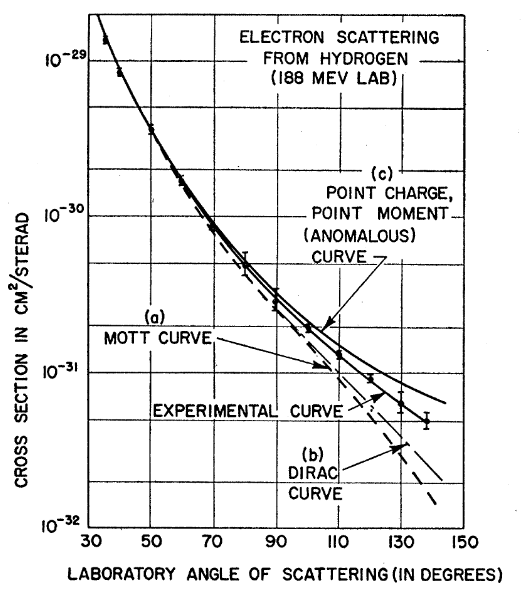
\includegraphics[width = 10cm]{mott_dirac_188mev}
    \caption{Holfstadter's 188MeV-electron scattering Experiment shows a deviation from the expected differential cross section of several theoretical models including the Mott Curve.}
    \label{fig:ruthenergy}
\end{figure}

The data collected by Hofstadter diverged from any of the point particle experimental models, even those that had corrective terms for the spin of the proton electron.

This deviation from predictions indicated that the electron was spending time inside of the proton, thus reducing the coulomb forces experienced between the proton and electron.
This was indication that the proton was of finite size. What remained was to quantifying that size.

For this Hofstadter built upon the research of M. N. Rosenbluth. Rosenbluth had further extended the Mott-Rutherford differential cross-section equation or use in a quantum system. See Equation \ref{eq:rosenbluth} for the cross-section of a diffuse proton\cite{McAllister1956}.

\begin{equation}\label{eq:rosenbluth}
\sigma = \sigma_{NS}{1 + \frac{q^2}{4M^2}[2(1+\mu)^2*\tan^2(\theta/2)+\mu^2]}
\end{equation}

\begin{equation}\label{Rosenbluth1950}
    \sigma_{NS} = \frac{e^4}{4E^2}(\frac{\cos^2(\theta/2)}{sin^4(\theta/2)}\frac{1}{1+(2E/M)sin^2(\theta/2)}
\end{equation}

\newcommand{\lambdabar}{{\mkern0.75mu\mathchar '26\mkern -9.75mu\lambda}}

\begin{equation}
    q = \frac{(2/\lambdabar)\sin(\theta/2)}{[1+(2E/M)sin^2(\theta/2)]^\frac{1}{2}}
\end{equation}

\begin{equation}\label{Rosenbluth1950}
    \sigma = \sigma_{NS}{F_1^2 + \frac{q^2}{4M^2}[2(F_1+\mu{F_2})^2*\tan^2(\theta/2)+\mu^2F_2^2]}
\end{equation}

Add descriptions of the equations and their terms. Think about this section for a while. What am I trying to achieve here? Do I just want to introduce the Rosenbluth equation, what good does this do for a new person trying to understand it. How do we go from this to a cross section/extract a form facter???




\bibliographystyle{plain}
\bibliography{simple}

\end{document}
  
